%%
%% This is file `main.tex`
%% modified from `sample-sigconf.tex',
%%
%% The original source files were:
%%
%% samples.dtx  (with options: `sigconf')
%% 
%% IMPORTANT NOTICE:
%% 
%% For the copyright see the source file.
%% 
%% Any modified versions of this file must be renamed
%% with new filenames distinct from sample-sigconf.tex.
%% 
%% For distribution of the original source see the terms
%% for copying and modification in the file samples.dtx.
%% 
%% This generated file may be distributed as long as the
%% original source files, as listed above, are part of the
%% same distribution. (The sources need not necessarily be
%% in the same archive or directory.)
%%https://www.overleaf.com/project/61ef0be310bca79def9de128
%%https://www.overleaf.com/project/61ef0be310bca79def9de128
%% Commands for TeXCount
%TC:macro \cite [option:text,text]
%TC:macro \citep [option:text,text]
%TC:macro \citet [option:text,text]
%TC:envir table 0 1
%TC:envir table* 0 1
%TC:envir tabular [ignore] word
%TC:envir displaymath 0 word
%TC:envir math 0 word
%TC:envir comment 0 0
%%
%%
%% The first command in your LaTeX source must be the \documentclass command.
%\documentclass[acmsmall]{acmart}
% \documentclass[acmsmall,screen,review]{acmart}
\documentclass[acmsmall,screen]{acmart}
%%
%% \BibTeX command to typeset BibTeX logo in the docs
\AtBeginDocument{%
  \providecommand\BibTeX{{%
    \normalfont B\kern-0.5em{\scshape i\kern-0.25em b}\kern-0.8em\TeX}}}

%% Rights management information.  This information is sent to you
%% when you complete the rights form.  These commands have SAMPLE
%% values in them; it is your responsibility as an author to replace
%% the commands and values with those provided to you when you
%% complete the rights form.

\copyrightyear{2022}
\acmYear{2022}
\setcopyright{acmcopyright}\acmConference[PEARC '22]{Practice and Experience in Advanced Research Computing}{July 10--14, 2022}{Boston, MA, USA}
\acmBooktitle{Practice and Experience in Advanced Research Computing (PEARC '22), July 10--14, 2022, Boston, MA, USA}
\acmPrice{15.00}
\acmDOI{10.1145/3491418.3535174}
\acmISBN{978-1-4503-9161-0/22/07}

%\usepackage{draftwatermark}
%\SetWatermarkText{Draft}
%\SetWatermarkScale{2}

%% These commands are for a PROCEEDINGS abstract or paper.
%% TODO Booktitle, Price, ISBN if necessary
% \acmConference[PEARC '22]{PEARC '22: Revolutionary: Computing, Connections, You}{July 10–-14, 2022}{Boston, MA, USA}
% \acmBooktitle{Woodstock '18: ACM Symposium on Neural Gaze Detection,
%   June 03--05, 2018, Woodstock, NY}
% \acmPrice{15.00}
%\acmISBN{978-1-4503-XXXX-X/18/06}


%%
%% Submission ID.
%% Use this when submitting an article to a sponsored event. You'll
%% receive a unique submission ID from the organizers
%% of the event, and this ID should be used as the parameter to this command.
%%\acmSubmissionID{123-A56-BU3}

%%
%% The majority of ACM publications use numbered citations and
%% references.  The command \citestyle{authoryear} switches to the
%% "author year" style.
%%
%% If you are preparing content for an event
%% sponsored by ACM SIGGRAPH, you must use the "author year" style of
%% citations and references.
%% Uncommenting
%% the next command will enable that style.
%%\citestyle{acmauthoryear}

%%
%% end of the preamble, start of the body of the document source.
\begin{document}

%%
%% The "title" command has an optional parameter,
%% allowing the author to define a "short title" to be used in page headers.
\title[Validating new AutoCV workflows to traditional AutoML]{Validating new Automated Computer Vision workflows to traditional Automated Machine Learning}
%% AUTOML
%%
%% The "author" command and its associated commands are used to define
%% the authors and their affiliations.
%% Of note is the shared affiliation of the first two authors, and the
%% "authornote" and "authornotemark" commands
%% used to denote shared contribution to the research.
%%

\author{Davin Lin}
\affiliation{%
  \institution{Grinnell College}
%%  \streetaddress{P.O. Box 4006}
  \city{Grinnell}
  \state{Iowa}
  \country{USA}
%%  \postcode{50112}
}
\email{lindavin@grinnell.edu}

%\orcid{1234-5678-9012}
\author{Padma Prabagaran}
\affiliation{%
% TODO Street Address
  \institution{Arizona State University}
  \city{Tempe}
  \state{Arizona}
  \country{USA}
%%  \postcode{85281}
}
\email{pprabaga@asu.edu}

\author{Dirk Colbry}
\affiliation{%
  \institution{Michigan State University}
  \city{East Lansing}
  \state{Michigan}
  \country{USA}
%%  \postcode{48824}
}
\email{colbrydi@msu.edu}


%%
%% By default, the full list of authors will be used in the page
%% headers. Often, this list is too long, and will overlap
%% other information printed in the page headers. This command allows
%% the author to define a more concise list
%% of authors' names for this purpose.
\renewcommand{\shortauthors}{Davin Lin, Padma Prabagaran, and Dirk Colbry}

%%
%% PEARC Call for Participation
%% https://pearc.acm.org/pearc22/call-for-participation/
%% Full Papers (Up to 12 pages as laid out in the single-column publication format, including references)
%% Short Papers (Up to 6 pages as laid out in the single-column publication format, including references) 
%%

%%
%% The abstract is a short summary of the work to be presented in the
%% article.
\begin{abstract}
This paper presents some experiments to validate the design of an Automated Computer Vision (AutoCV) library for applications in scientific image understanding.  AutoCV attempts to define a search space of algorithms used in common image analysis workflows and then uses a fitness function to automatically select individual algorithmic workflows for a given problem.  The final goal is a semi-automated system that can assist researchers in finding specific computer vision algorithms that work for their specific research questions. As an example of this method the researchers have built the SEE-Insight tool which uses genetic algorithms to search for image analysis workflows. This tool has been used to implement an image segmentation workflow (SEE-Segment) and is being updated and modified to work with other image analysis workflows such as anchor point detection and counting.  This work is motivated by analogous work being done in Automated Machine Learning (AutoML).  As a way to validate the approach, this paper uses the SEE-Insight tool to recreate an AutoML solution (called SEE-Classify) and compares results to an existing AutoML solution (TPOT).  As expected the existing AutoML tool worked better than the prototype SEE-Classify tool.  However, the goal of this work was to learn from these well-established tools and possibly identify one of them that could be modified as a mature replacement for the core SEE-Insight search algorithm. Although this drop-in replacement was not found, reproducing the AutoML experiments in the SEE-Insight framework provided quite a few insights into best practices for moving forward with this research. 

%  This work validates the design of the SEE-Insight Genetic algorithm (GA) algorithm selection tool.  Although SEE-Insight is intended to search for solutions to scientific image annotation problems it is highly extensible and can easily be adopted to search other algorithm/hyperparameter spaces.  To validate the design of the software this work implements a AutoML tool using the SEE-Insight framework.  Although not intended as a replacement this work demonstrates that the results of running using the SEE-Insight meta-learning system is comparable to Auto-Sklearn, TPOP and GAMA, the current state of the art in AuotoML. This work is intended to be a proof-of-concept of the SEE-Insight search algorithm and the first step in validating this approach.
\end{abstract}

%%
%% The code below is generated by the tool at http://dl.acm.org/ccs.cfm.
%% Please copy and paste the code instead of the example below.
%%
%% TODO
\begin{CCSXML}
<ccs2012>
<concept>
<concept_id>10011007.10011006.10011072</concept_id>
<concept_desc>Software and its engineering~Software libraries and repositories</concept_desc>
<concept_significance>500</concept_significance>
</concept>
</ccs2012>
\end{CCSXML}

\ccsdesc[500]{Software and its engineering~Software libraries and repositories}

%%
%% Keywords. The author(s) should pick words that accurately describe
%% the work being presented. Separate the keywords with commas.
%% TODO
\keywords{datasets, neural networks, gaze detection, text tagging}

%%
%% This command processes the author and affiliation and title
%% information and builds the first part of the formatted document.
\maketitle

\section{Introduction}


%% Some of this can go into related works maybe?

Both AutoML and AutoCV are instances of the Combined Algorithm Selection and Hyperparameter optimization problem (CASH) \cite{Feurer2019}, where the algorithm choice is treated as an additional search parameter. AutoML software such as autosklearn \cite{feurer-neurips15a} address the CASH problem by utilizing Bayesian Optimization to perform guided search over and construct fixed machine learning pipelines (consisting of data pre-processors, feature selectors, and machine learning algorithms). It also takes it a step further by using Meta-learning to warmstart the Bayesian Optimization algorithm and using an offline automated ensemble construction method to optimize classification performance. Another example of AutoML, TPOT \cite{le2020scaling}  uses a tree based hierarchy and Genetic Programming to optimize machine learning pipelines and tries to maximize classification performance while minimizing the size of the tree pipeline. 


To our knowledge, unlike AutoML,  there is no CASH implementation of an AutoCV pipeline. To that end, SEE-Insight was built using a genetic algorithm to address the CASH problem for AutoCV. The core data structures and algorithms within SEE-Insight software are intended to be algorithm agnostic and only require vectorization of the search space (both algorithms and hyperparameters) and a problem specific fitness function.  The search space is intended to be extendable into any problem space with these two factors. Since SEE-Insight is the first to attempt for an AutoCV solution it is difficult to compare the results of the search algorithm with existing approaches. The work presented in this paper evaluates the effectiveness of the SEE-Insight genetic search algorithm by implementing an AutoML system (called SEE-Classify) and comparing the results to well established algorithms such as TPOT. The SEE-Insight software framework was easily adapted to this specific problem and provides a direct way to validate the software framework and learn from these well established solutions before moving into the more complex AutoCV workflows.
%for which there are no existing software we can use to validate the approach.


%% Update: TPOT on Segment dataset, figures...ROC_AUC
%% median ROC curve?
%% box-plot with 20-80% for AUC scores
%% 
%% Davin has Questions about GP terminology and how TPOT works...
%% 95% CI for cross-validation runs
%% Run comparisons with Auto-sklearn
%%
%% Davin plans to add experiments for these datasets:
%% 1. riccardo (too large): https://www.openml.org/d/41161 ; 4297 features; 20000 rows
%% 2. guillermo (too large): https://www.openml.org/d/41159; 4297 features; 20000 rows
%% phoneme (done), nasal or oral: https://www.openml.org/d/1489; 5 features; 5040 rows
%% kc1 (done), software detection: https://www.openml.org/d/1067; 21 features; 2109 rows
%%

\section{Method} 

\subsection{Genetic algorithm (GA)} The core of this approach is a simple genetic algorithm (See Figure \ref{fig:ga-flow}). First, a population of individuals is randomly generated. The $N$ best individuals (10 in this example) are selected via the fitness function and crossover and mutation is performed on the best individuals to create one portion of the population of the next generation. The remaining portion of the population is randomly generated. This process of selection, crossover, mutation, and random generation continues in a loop and GA terminates after reaching a specified number of iterations (i.e. "generations").

\begin{figure}[h]
  \centering
  %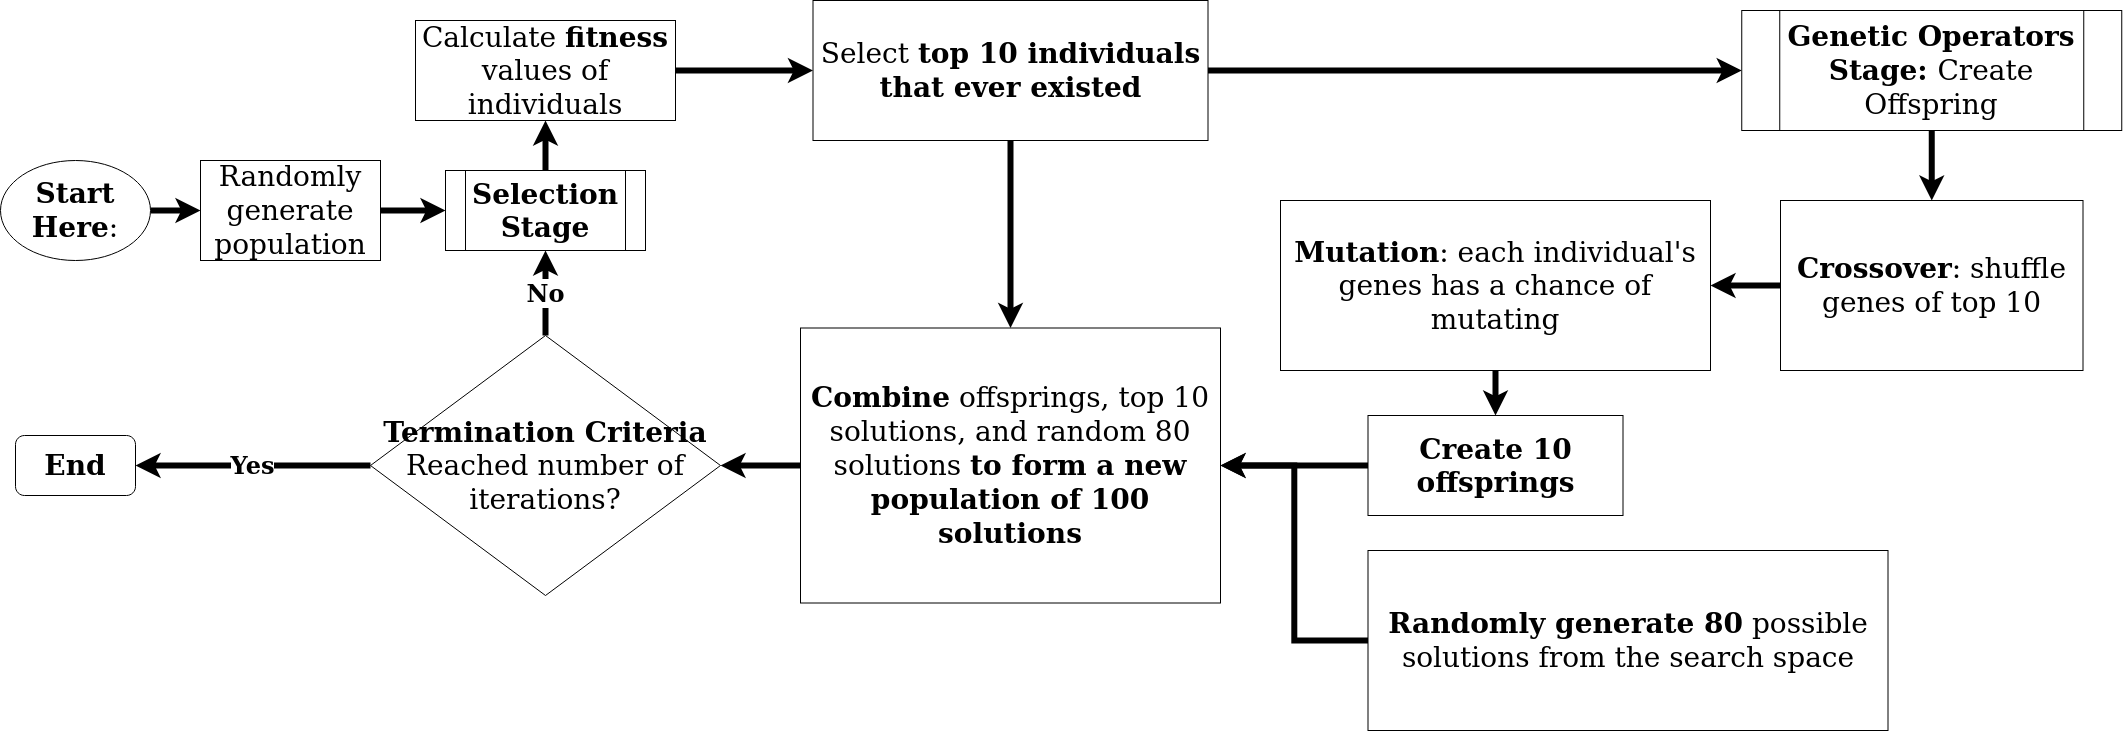
\includegraphics[width=13.5cm]{flowcharts/ga-flow.drawio.png}
  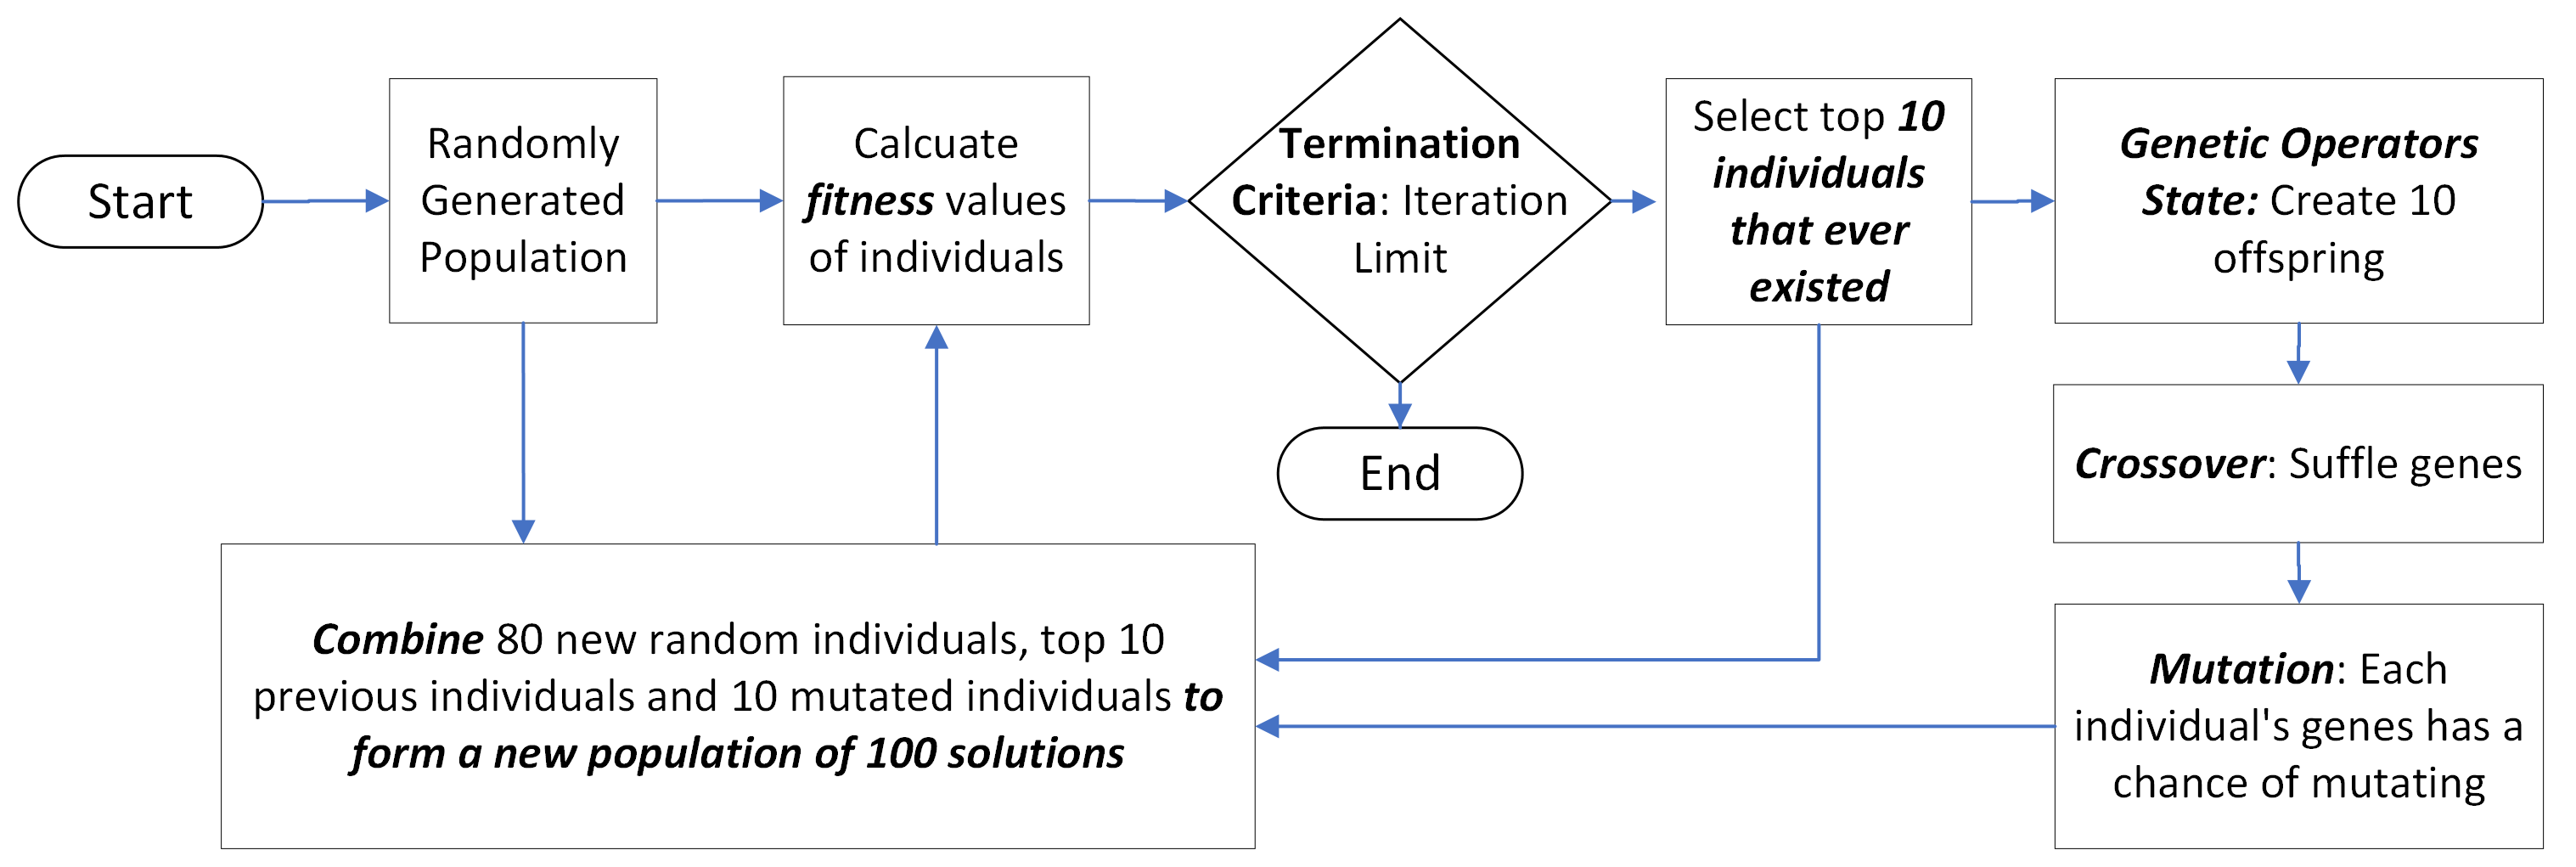
\includegraphics[width=14cm]{flowcharts/New_Diagram.png}
  \caption{Genetic algorithm outline}
  \label{fig:ga-flow}
\end{figure}

Individuals are represented as a vector of values where all hyperparameters are included (See Figure \ref{fig:representation}). Because of this representation, algorithm lists are "bloated" in that they contain values that will not be used when converting the individual into an ML pipeline via scikit-learn. Crossover is performed by swapping one random contiguous section of each algorithm list. Mutation is performed by re-sampling a hyperparameter value from its corresponding range of possible values. This work uses the default mutation rate and crossover rates in See-Segment which are both 0.9.

\begin{figure}[h]
  \centering
  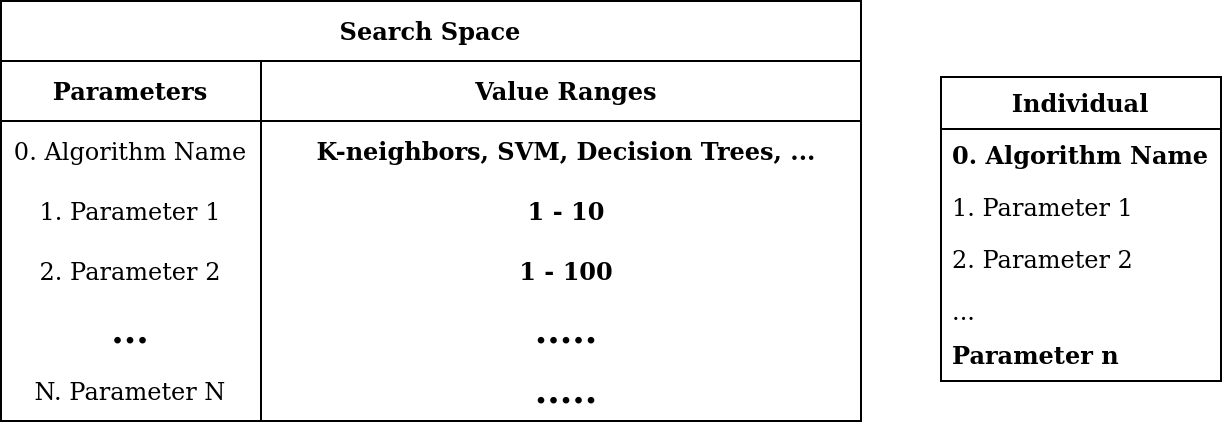
\includegraphics[width=10cm]{flowcharts/see-classify-algo-representation-list represetation.drawio.png}
  \caption{Search space and individual representation}
  \label{fig:representation}
\end{figure}
\subsection{Search space} The search space for the GA is a subset of the algorithms implemented in the scikit-learn library. Points in the search space are called individuals and are represented as a vector of values where all hyperparameters are included (See Figure \ref{fig:representation}). This search space currently consists of the following supervised learning classification algorithms and some of their hyperparameters: Ada Boost, Decision Trees, Extra Trees, Gaussian Naive Bayes, Gaussian Process, Gradient Boosting, K Nearest Neighbors, Linear Discriminant Analysis, Logistic Regression, Neural Networks, Quadratic Discriminant Analysis, Random Forest, and Support Vector Classification. This GA and search space implementation does not yet support multiple pipeline operators such as including preprocessors or feature selectors.
%% Davin moved the explanation of the search space with the table of hyperparameters to the ./old_text.tex file.
\subsection{Fitness function} 
To evaluate an individual, its corresponding vector is used to construct a machine learning model via the corresponding algorithm and hyperparameters implemented in scikit-learn. This work used the stratified 10-fold cross-validation scheme to evaluate the constructed pipeline on a given set of data. Since the SEE-Insight framework minimizes an individual's fitness, in SEE-Classify the fitness of an individual is $1 - \text{"10-fold cross-validated accuracy"}$. The accuracy metric this work uses in each fold of stratified 10-fold cross validation is the ratio: $\frac{\text{\# correct labels}}{\text{total \# of items in dataset}}$. The SEE-Classify tool is designed such that it should be relatively simple to swap out fitness functions which will be an area of future work.

\subsection{Data and computational resources}
This work compared the performance of TPOT, and SEE-Classify (the SEE-Insight implementation of an AutoML solution) by testing the two systems on four benchmark datasets. This work used the real world binary classification datasets Wisconsin Breast Cancer Diagnostic (wbcd) \cite{misc_breast_cancer_wisconsin_(diagnostic)_17}, blood transfusion \cite{misc_blood_transfusion_service_center_176}, phoneme, and kc1 \cite{Sayyad-Shirabad+Menzies:2005}; the latter three were selected from an Open source OpenML AutoML benchmark \cite{amlb2019}. For simplicity, these datasets were chosen because they consisted only of numerical features and were not missing any values.

%% phoneme dataset did not have a citation requirement in the OpenML site; https://new.openml.org/search?type=data&sort=runs&id=1489&status=active; it has a source, but I figure out who to properly cite.

All experiments were run on  High Performance Computer Center ({HPCC}) at the Michigan State University ({MSU}) Institute for Cyber-Enabled Research ({ICER}). The experiments were conducted in a pleasantly parallel way using job arrays with different input seeds on cores across the cluster. Each job searches a different part of the overall search space with the best results easily determined by reviewing the output of all runs for the lowest fitness value.  % In these experiments each core consisted of an Intel(R) Xeon(R) CPU E5-2670 v2 @ 2.50GHz. 


% pair the tpot and sklearn movement of best solution so far.

% \subsection{Scikit-learn tutorial}

% Figure \ref{fig:scikit_learn_ga} plots the population mean and the mean of the top 10 solutions found by generation number averaged over the 100 runs of the GA. The shaded regions are two standard deviations from the averages. This shows that the GA was able to rapidly converge onto the best models specified in the tutorial.

%% Davin: If there's time, we could look into Nested-Cross-Validation; it looks similar to what we're doing here; I just don't understand all the details.... https://machinelearningmastery.com/nested-cross-validation-for-machine-learning-with-python/

%% Davin: Is it clear that the random states used to split data for TPOT and and for SEE are not necessarily the same?
% Points in the search space are called individual and are represented as a vector of values where all hyperparameters are included (See Figure \ref{fig:representation}).
For each AutoML system, the following experiment is repeated 30 times with a unique random seed for each dataset (See Figure \ref{fig:experimen_workflow}). Following the methodology outlined in the TPOT experiment \cite{le2020scaling}, each dataset is randomly split into a stratified 75\% training and 25\% validation set (i.e the "Splitter" step). The training set is used by the AutoML system to search for an optimal classification pipeline. The cross-validation scheme used in the fitness function further splits the training set into a stratified 75\%/25\% training/testing set. The validation set is used to evaluate the optimal or best ML pipeline found so far in a specified time budget.

\section{Results}
\begin{figure}[h]
  \centering
  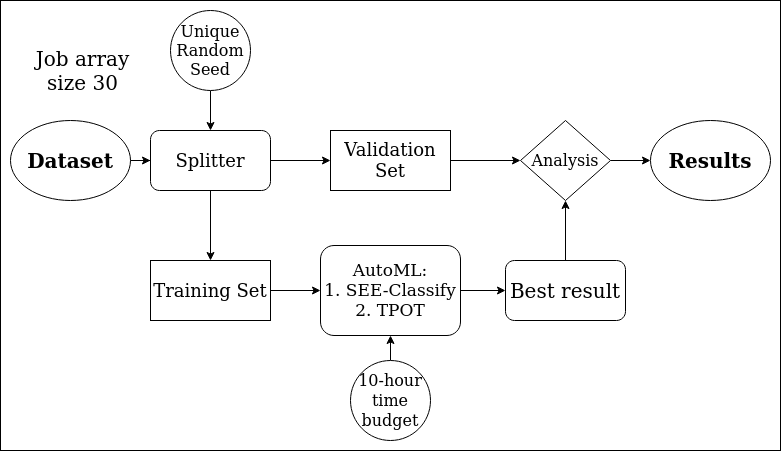
\includegraphics[width=9cm]{flowcharts/experiment_flow_horizontal.png}
  \caption{Experiment workflow}
  \label{fig:experimen_workflow}
\end{figure}

This work compared TPOT with SEE-Classify using a 10-hour time budget. In TPOT, time budgets are supported by default; whereas for SEE-Classify the SLURM workload manager is used to interrupt the process after 10 hours. The best found solution by SEE-Classify is analyzed offline and if its GA had been interrupted during a generation, that generation is ignored in this analysis. This SEE-Classify implementation does not use the same data pre-processors as TPOT, Instead this work only uses a simple normalization.  Although it is possible to include these pre-processors they are not necessary to validate the performance of the core algorithm.  

%%TODO What is a "Standard Scalar".  I'm not sure I understand this term.

The ROC (Receiver Operator Curves) of the best ML pipelines found by both systems are (See Figure \ref{fig:roc}), with TPOT pipelines having a slightly larger but comparable AUC (Area Under the Curve) for the wbcd, phoneme, and kc1 datasets (See Figure \ref{fig:auc}). The training and validation accuracy are also similar between the two systems as shown in \ref{fig:train_valid}. Interestingly, optimal pipelines found by SEE-Classify tend to experience less degradation in validation accuracy across the four datasets, with a maximum of 8\% decrease compared to 10\% for the blood transfusion dataset (See Figure \ref{fig:percent_decrease}).


\begin{figure}[h]
  \centering
  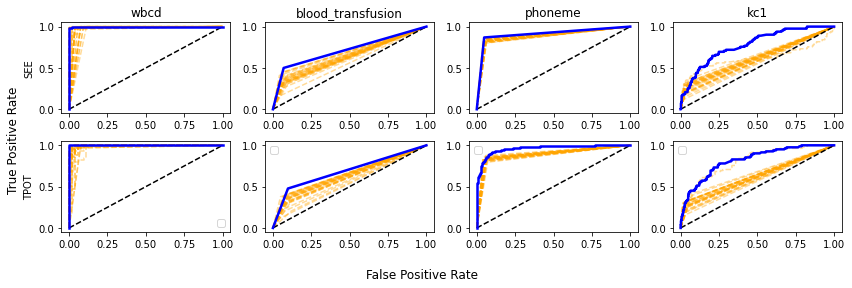
\includegraphics[width=13cm]{figures_2/roc_see_tpot_4.png}
  \caption{ROC curves of TPOT vs SEE}
  \label{fig:roc}
\end{figure}


\begin{figure}[h]
  \centering
  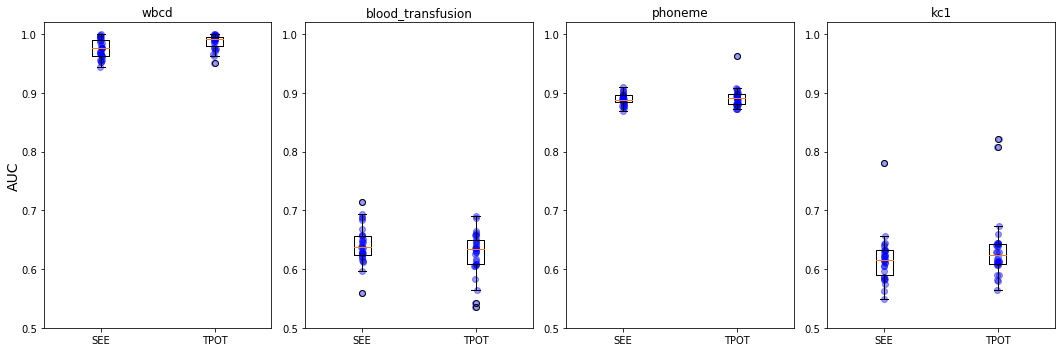
\includegraphics[width=13cm]{figures_2/auc_see_tpot_4.png}
  \caption{The AUC of TPOT and SEE. Each plot represents 30 repeated experiments, with the inner line as the median, the ends as the 25th and 75th quartiles, and the circled dots as outliers.}
  \label{fig:auc}
\end{figure}

\begin{figure}[h]
  \centering
  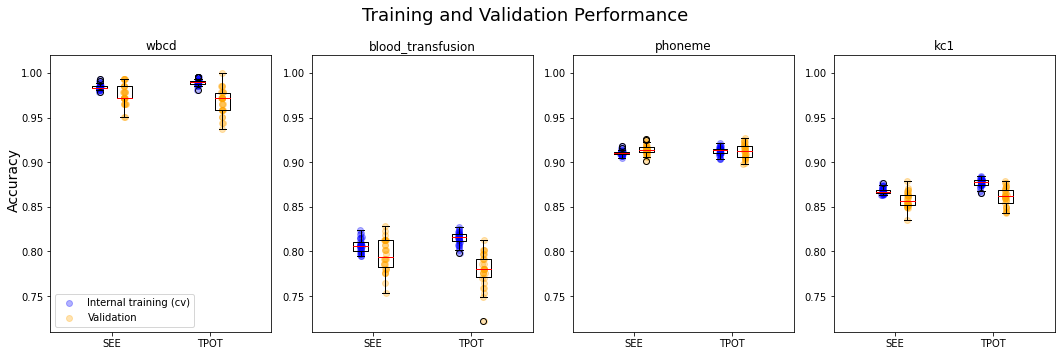
\includegraphics[width=13cm]{figures_2/see_tpot_train_valid.png}
  \caption{The training and validation accuracy of TPOT and SEE. Each plot represents 30 repeated experiments, with the inner line as the median, the ends as the 25th and 75th quartiles, and the circled dots as outliers.}
  \label{fig:train_valid}
\end{figure}


\begin{figure}[h]
  \centering
  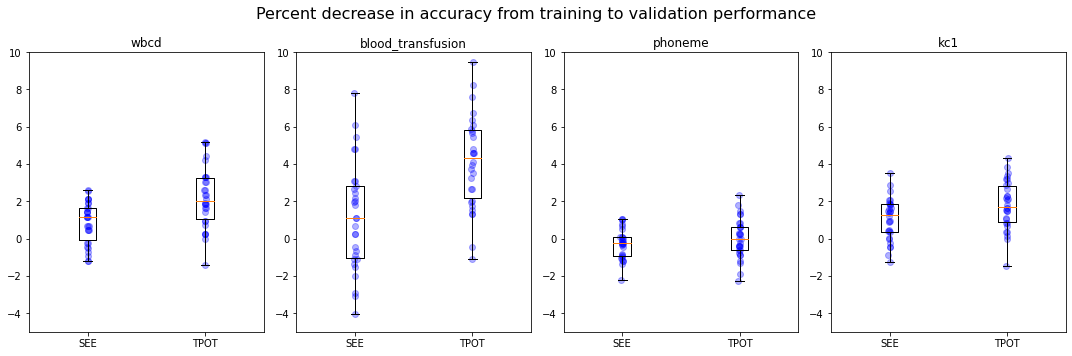
\includegraphics[width=13cm]{figures_2/percent_drop_see_tpot_4.png}
  \caption{The percent decrease in accuracy of TPOT and SEE from training to validation. Each plot represents 30 repeated experiments, with the inner line as the median, the ends as the 25th and 75th quartiles, and the circled dots as outliers.}
  \label{fig:percent_decrease}
\end{figure}
As a verification of its GA, Figure \ref{fig:median} shows that the median training accuracy of SEE-Classify increases with TPOT's early on; however, growth stops much earlier in SEE-Classify. Figure \ref{fig:median} further shows that SEE-Classify has comparable, although weaker, performance with TPOT because difference in median training accuracy is never greater than 2.5\%. However, for the larger datasets Phoneme and kc1, TPOT's algorithm processes many more individual's than does SEE-Classify.

\begin{figure}[h]
  \centering
  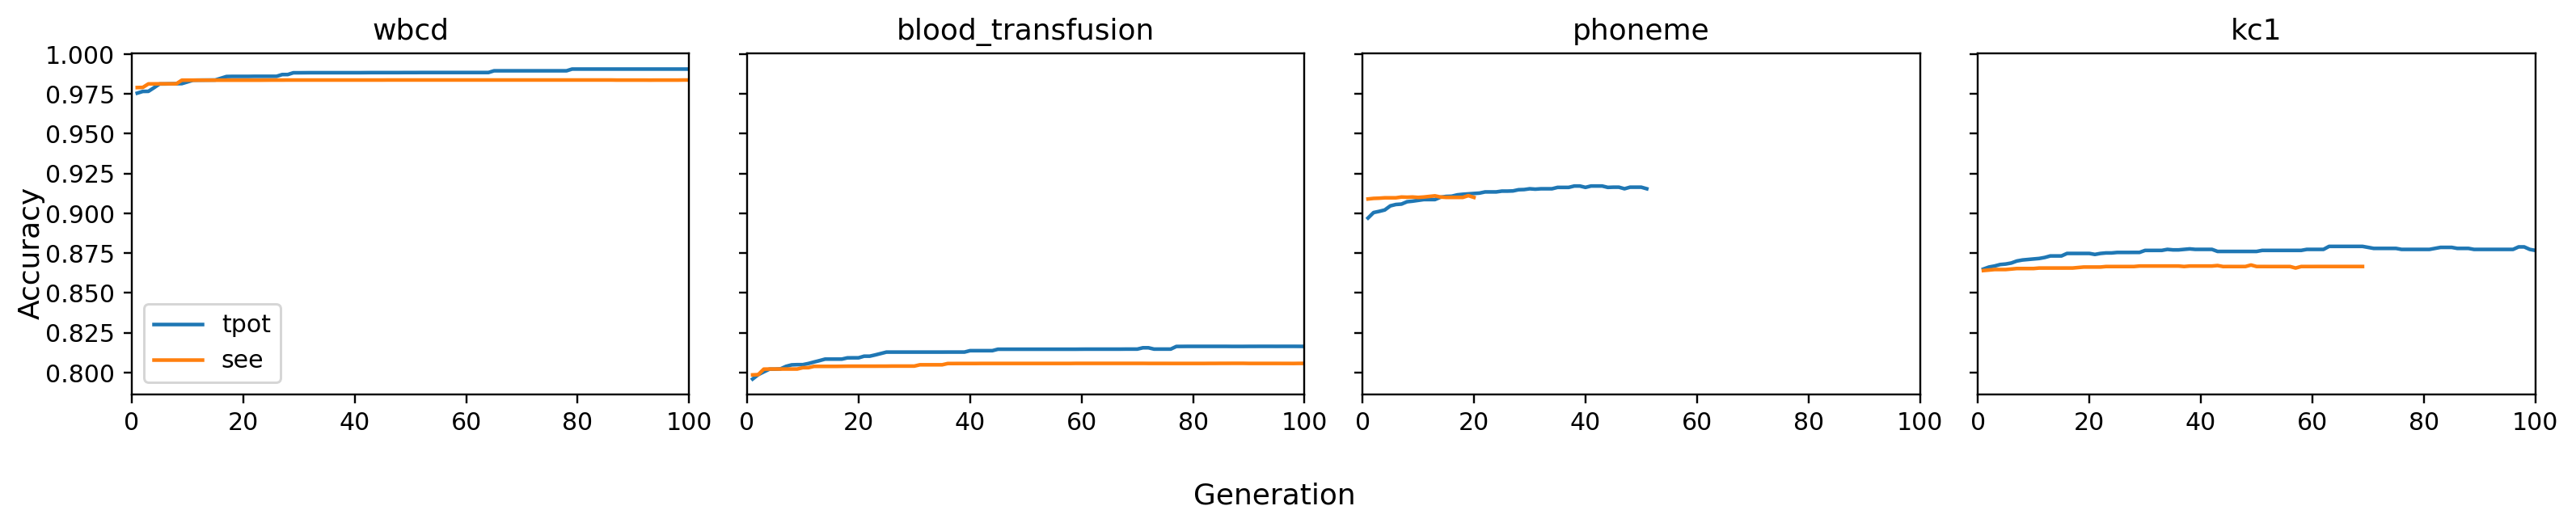
\includegraphics[width=14cm]{figures_2/see_tpot_median.png}
  \caption{The median accuracy across experiments of the best individual individual of each generation. When calculating the median, generation numbers that the GA/GP did not finish or reach are ignored.}
  \label{fig:median}
\end{figure}

\section{Concluding discussion}
%This paper presents a AutoML tool (called SEE-Classify) which uses a simple Genetic Algorithm (GA) developed for Automated Computer Vision (AutoCV) workflows.  
AutoML tools search the hyperparameter space of multiple classification algorithms to find the best parameters for particular problems. The purpose of this research was not to reinvent the wheel, instead, the goals of conducting these tests were to a) validate the underlying SEE-Insight GA by comparing results to well-established AutoML solutions and b) gain insight and best practices for improving the SEE-Insight core algorithms.  Experimental results show that the SEE-Classify algorithm is able to converge to similar solutions that reproduce the prior work. A secondary goal was to evaluate the existing AutoML software to see if they could be adapted as a drop-in replacement for the AutoCV research. Unfortunately a simple drop-in solution was not found and it is an area of future work for the researchers to continue to explore how the TPOT software could be adapted to this new problem domain.  All of the SEE-Classify software has been released and incorporated into the SEE-Segment project \cite{see-segment}, which is provided under an open source license on GitHub, and researchers are encouraged to try the software and contribute to the project. 

\begin{acks}
%% TODO Acknowledgements
We would like to acknowledge the HPCC at MSU ICER, the ICER ACRES Summer REU Program (NSF OAC \#1949912), and the XSEDE EMPOWER Program (NSF OAC \#1053575) for their support and funding in this research.

\end{acks}

%%
%% The next two lines define the bibliography style to be used, and
%% the bibliography file.
\bibliographystyle{ACM-Reference-Format}

\bibliography{my_library}

%%
%% END OF DOCUMENT
%%
%% The information below are tips on doing
%% tables and the appendix taken from the 
%% original template.
%%

% \section{Tables}

% The ``\verb|acmart|'' document class includes the ``\verb|booktabs|''
% package --- \url{https://ctan.org/pkg/booktabs} --- for preparing
% high-quality tables.

% Table captions are placed {\itshape above} the table.

% Because tables cannot be split across pages, the best placement for
% them is typically the top of the page nearest their initial cite.  To
% ensure this proper ``floating'' placement of tables, use the
% environment \textbf{table} to enclose the table's contents and the
% table caption.  The contents of the table itself must go in the
% \textbf{tabular} environment, to be aligned properly in rows and
% columns, with the desired horizontal and vertical rules.  Again,
% detailed instructions on \textbf{tabular} material are found in the
% \textit{\LaTeX\ User's Guide}.

% Immediately following this sentence is the point at which
% Table~\ref{tab:freq} is included in the input file; compare the
% placement of the table here with the table in the printed output of
% this document.

% \begin{table}
%   \caption{Frequency of Special Characters}
%   \label{tab:freq}
%   \begin{tabular}{ccl}
%     \toprule
%     Non-English or Math&Frequency&Comments\\
%     \midrule
%     \O & 1 in 1,000& For Swedish names\\
%     $\pi$ & 1 in 5& Common in math\\
%     \$ & 4 in 5 & Used in business\\
%     $\Psi^2_1$ & 1 in 40,000& Unexplained usage\\
%   \bottomrule
% \end{tabular}
% \end{table}

% To set a wider table, which takes up the whole width of the page's
% live area, use the environment \textbf{table*} to enclose the table's
% contents and the table caption.  As with a single-column table, this
% wide table will ``float'' to a location deemed more
% desirable. Immediately following this sentence is the point at which
% Table~\ref{tab:commands} is included in the input file; again, it is
% instructive to compare the placement of the table here with the table
% in the printed output of this document.

% \begin{table*}
%   \caption{Some Typical Commands}
%   \label{tab:commands}
%   \begin{tabular}{ccl}
%     \toprule
%     Command &A Number & Comments\\
%     \midrule
%     \texttt{{\char'134}author} & 100& Author \\
%     \texttt{{\char'134}table}& 300 & For tables\\
%     \texttt{{\char'134}table*}& 400& For wider tables\\
%     \bottomrule
%   \end{tabular}
% \end{table*}

% Always use midrule to separate table header rows from data rows, and
% use it only for this purpose. This enables assistive technologies to
% recognise table headers and support their users in navigating tables
% more easily.

%%
%% If your work has an appendix, this is the place to put it.
% \appendix

% \section{Research Methods}

% \subsection{Part One}

% Lorem ipsum dolor sit amet, consectetur adipiscing elit. Morbi
% malesuada, quam in pulvinar varius, metus nunc fermentum urna, id
% sollicitudin purus odio sit amet enim. Aliquam ullamcorper eu ipsum
% vel mollis. Curabitur quis dictum nisl. Phasellus vel semper risus, et
% lacinia dolor. Integer ultricies commodo sem nec semper.

% \subsection{Part Two}

% Etiam commodo feugiat nisl pulvinar pellentesque. Etiam auctor sodales
% ligula, non varius nibh pulvinar semper. Suspendisse nec lectus non
% ipsum convallis congue hendrerit vitae sapien. Donec at laoreet
% eros. Vivamus non purus placerat, scelerisque diam eu, cursus
% ante. Etiam aliquam tortor auctor efficitur mattis.

% \section{Online Resources}

% Nam id fermentum dui. Suspendisse sagittis tortor a nulla mollis, in
% pulvinar ex pretium. Sed interdum orci quis metus euismod, et sagittis
% enim maximus. Vestibulum gravida massa ut felis suscipit
% congue. Quisque mattis elit a risus ultrices commodo venenatis eget
% dui. Etiam sagittis eleifend elementum.

% Nam interdum magna at lectus dignissim, ac dignissim lorem
% rhoncus. Maecenas eu arcu ac neque placerat aliquam. Nunc pulvinar
% massa et mattis lacinia.

\end{document}
\endinput
%%
%% End of file `main.txt`.
%% Modified from `sample-sigconf.tex'.
